%==============================================================================
% Sjabloon poster bachproef
%==============================================================================
% Gebaseerd op document class `a0poster' door Gerlinde Kettl en Matthias Weiser
% Aangepast voor gebruik aan HOGENT door Jens Buysse en Bert Van Vreckem

\documentclass[a0,portrait]{hogent-poster}

% Info over de opleiding
\course{Bachelorproef}
\studyprogramme{toegepaste informatica}
\academicyear{2024-2025}
\institution{Hogeschool Gent, Valentin Vaerwyckweg 1, 9000 Gent}

% Info over de bachelorproef
\title{De impact van mobiele netwerken op facilitair beheer: een vergelijkende studie van 4G en privaat 5G voor HOGENT}
%\subtitle{Ondertitel (eventueel)}
\author{Jan De Somviele}
\email{jan.desomviele@student.hogent.be}
\supervisor{Lena De Mol, Chantal Teerlinck}
\cosupervisor{Giselle Vercauteren (HOGENT)}

% Indien ingevuld, wordt deze informatie toegevoegd aan het einde van de
% abstract. Zet in commentaar als je dit niet wilt.
\specialisation{Systeem- en Netwerkbeheer}
\keywords{5G, 4G, gebouwbeheer}
\projectrepo{https://github.com/JanDeSomviele/Bachelorproef2025}

\begin{document}

\maketitle

\begin{abstract}
Deze poster onderzoekt de prestaties en betrouwbaarheid van 4G- en privaat 5G-netwerken in de context van gebouwbeheersystemen zoals verlichting en HVAC. Via netwerkmetingen en functionele testen worden de praktische implicaties en geschiktheid van mobiele netwerken binnen smart buildings geëvalueerd.
\end{abstract}

\begin{multicols}{2} % This is how many columns your poster will be broken into, a portrait poster is generally split into 2 columns

\section{Introductie}

In deze bachelorproef werd onderzocht hoe 4G en privaat 5G-netwerken presteren binnen het kader van een gebouwbeheersysteem (GBS), met toepassingen zoals verlichting en HVAC. De centrale onderzoeksvraag luidde: \textit{Wat is het verschil tussen 4G en privaat 5G in verband met prestaties en betrouwbaarheid van toepassingen binnen een GBS?}

Om de testen uit te voeren werden 2 opstellingen gebruikt. De eerste opstelling gebruikt een rasberry pi in plaats van een AS-P controller. De tweedde opstelling maakt gebruik van een Philips hue Bridge en lamp om een use case van verlichting te testen. %TO DO: anders verwoorden

\begin{center}
    \captionsetup{type=figure}
    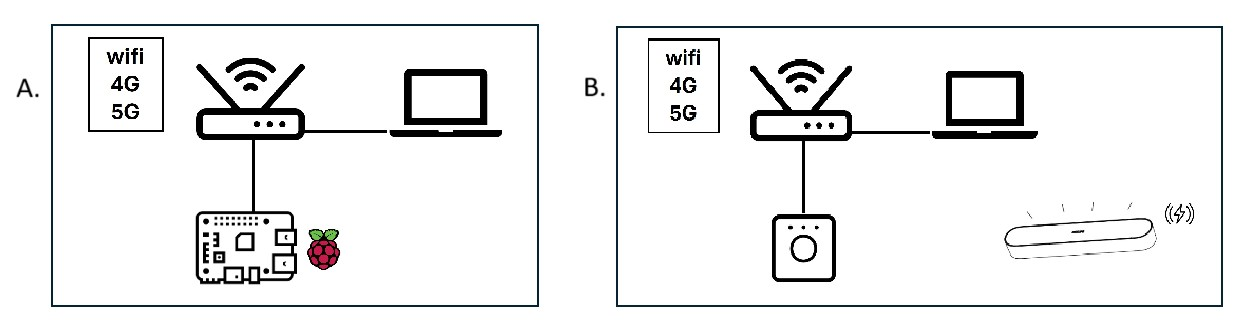
\includegraphics[width=0.45\textwidth]{../graphics/beideOpstellingen.jpg}
    \captionof{figure}{Opstelling A: , Opstelling B:}
\end{center}

\section{Experimenten}

\begin{center}
    \captionsetup{type=figure}
    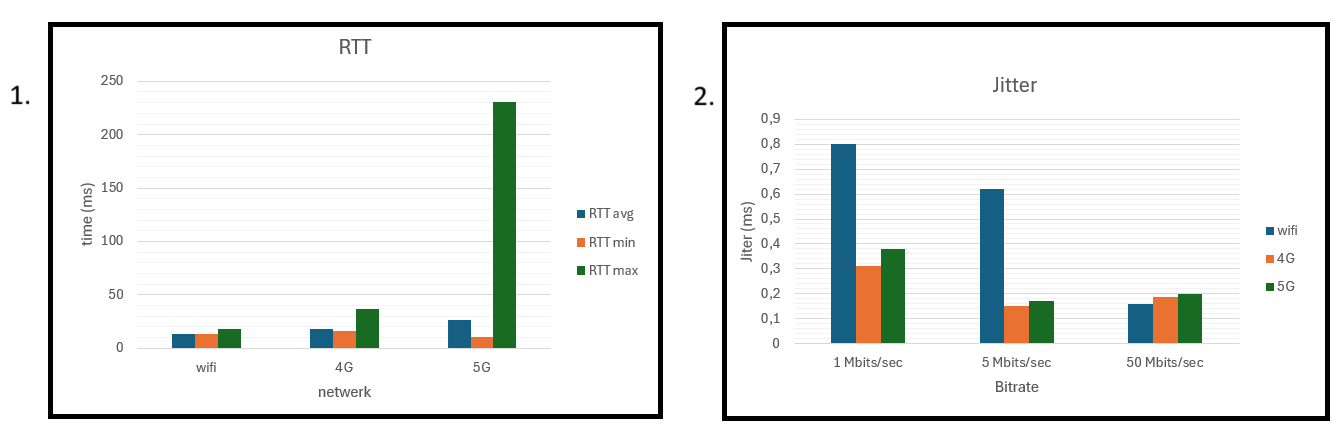
\includegraphics[width=0.45\textwidth]{../graphics/Latency-Jitter-grafiek.png}
    \captionof{figure}{Grafiek 1: , Grafiek 2:}
\end{center}

\begin{multicols}{2}
\subsection*{Latency}
latency + rtt uitleg. ping test 250 x 4 uitgevoerd per netwerk. grafiek 1 resultaten + uitleg
\subsection*{Jitter}
Jitter uitleg. iperf3-udp test 4x 2 min + 1,5,50 Mbit per netwerk met pc als iperf server. grafiek 2 + uitleg.
\end{multicols}
\subsection*{Packet loss}
ping test van latency + UDP iperf test van jitter. resultaten = geen packet loss bij elk netwerk.

\begin{center}
    \captionsetup{type=figure}
    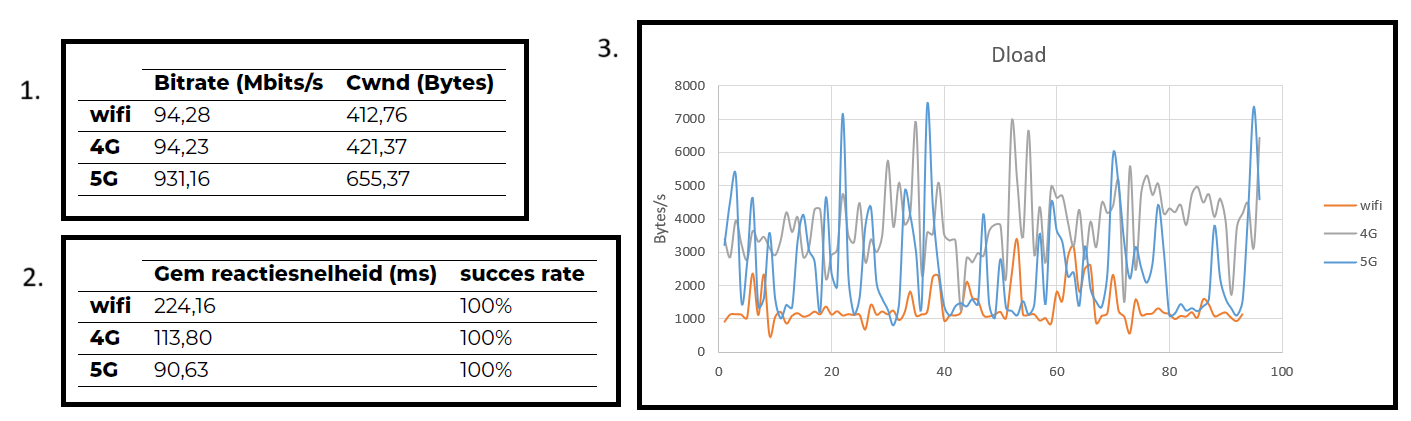
\includegraphics[width=0.45\textwidth]{../graphics/bandbreedteLichtHttp.png}
    \captionof{figure}{Tabel 1: bandbreedte , Tabel 2: licht, Grafiek 3: Download http test}
\end{center}

\begin{multicols}{2}
\subsection*{Bandbreedte}
iperf TCP test 4x2min per netwerk. uitleg resultaten

\subsection*{licht}
licht opstelling b. test 200 aan/uit x2 per netwerk. tabel = gem waarden + uitleg resultaten. 
\end{multicols}

\subsection*{http}
http = node red test van een curl naar een http endpoint op pc. grafiek is van de download van de test, uitleg resultaten.
\section{Conclusies}

5G bleek uit te blinken in throughput (tot 900 Mbit/s) en had bij lichte belasting zeer snelle reacties. Echter, 4G bood meer constante prestaties qua latency en betrouwbaarheid. In functionele testen (zoals lichtbediening) bleek 4G consistenter, terwijl 5G gevoeliger was voor fluctuaties. Wi-Fi presteerde wisselvalliger.

Mobiele netwerken zijn technisch geschikt voor GBS-toepassingen, mits rekening wordt gehouden met latentie, jitter en redundantie. Private 5G biedt bijkomende voordelen zoals QoS en interne netwerkcontrole.

\section{Toekomstig onderzoek}

Een herhaling van de testen in een private 5G-opstelling met SLA-garanties zou zinvol zijn. Verder onderzoek kan zich ook richten op schaalbaarheid bij honderden apparaten, energieverbruik van mobiele modules en de impact van netwerkcongestie of roaming binnen grote gebouwen.

\end{multicols}
\end{document}